% mainfile: ../../main.tex
\chapter{Filter functions from random sampling}\label{ch:ff:validation}
\AutoLettrine{In} our derivation of the average error map \liouvUeavg, \cref{eq:ff:cumulant_expansion}, we employed the cumulant expansion due to \citet{Kubo1962,Kubo1963}.
In his papers, \citeauthor{Kubo1962} makes the claim that this expansion is exact for Gaussian noise when truncating after the second order, even for \emph{$q$-numbers}, \ie, linear operators.
For \emph{$c$-numbers} -- scalars -- this is a well-known result in statistics; the Gaussian probability distribution is fully described by its first two cumulants, the mean $\mu$ and variance $\sigma^2$.
However, \citet{Fox1976} showed many years later that \citeauthor{Kubo1962}'s claim for $q$-numbers does not hold, and that non-commutativity in the Gaussian variables can cause higher-order cumulants to not vanish.
There are two limiting cases in which the expansion remains exact; first, for white noise, whose auto-correlation function is singular at $t=0$, and thus \enquote{decouples} higher-order cumulants, and second, commuting noise, for which $\comm{\Hc(t)}{\Hn(t)} = 0\forall t$.
Beyond these two cases, we must therefore assume that the map given by \cref{eq:ff:cumulant_expansion} is merely approximate when including only up to second-order terms from the Magnus expansion.\sidenote{
    Note that the cluster property still holds in all cases, and hence for Gaussian noise only even-order cumulants do not vanish~\cite{VanKampen1974,VanKampen1974a,Fox1976,Bianucci2020}.
}
In this chapter, we investigate the extent of this error.
To this end, we compute the \emph{exact} \acrfull{ff} using a \acrfull{mc} approach by randomly sampling monochromatic noise fields.

\section{Reconstruction by frequency-comb time domain simulation}\label{sec:ff:validation:method}
For a given interaction-picture quantum operation \liouvUetavg resulting from the quantum system's evolution under the noise fully characterized by its \gls{psd} $S(\omega)$, we \emph{define} the filter function \FFot by
\begin{align}\label{eq:ff:filter_function:definition}
    \liouvUetavg = \exp\cumulantfun(\tau) = \exp\left\{-\int\frac{\dd{\omega}}{2\pi}\FFot S(\omega)\right\}.
\end{align}
Now, suppose that
\begin{equation}\label{eq:ff:psd:monochromatic}
    S(\omega) = 2\pi\sigma_i^2 \delta(\omega - \omega_i) \eqqcolon S_i(\omega),
\end{equation}
that is, the \gls{psd} of a monochromatic sinusoid of frequency $\omega_i$ and \gls{rms} $\sigma_i$.\sidenote{
    \Cref{eq:ff:psd:monochromatic} discretizes $S(\omega)$ by sampling it at points $\omega_i$, \ie,
    \begin{align*}
        S(\omega) \sim \lim_{n\to\infty}\sum_{i=1}^n S_i(\omega).
    \end{align*}
    See also \cref{sidenote:continuum_limit}.
}
\Cref{eq:ff:filter_function:definition} then becomes
\begin{align}
    \ev*{\liouvUe_i(\tau)} \coloneqq \liouvUetavg =& \exp\left\lbrace -2\pi\sigma_i^2\int\frac{\dd{\omega}}{2\pi}\FFot\delta(\omega - \omega_i)\right\rbrace \\
                                                  =& \exp\left\lbrace -\sigma_i^2\mc{F}(\omega_i;\tau)\right\rbrace, \label{eq:ff:filter_function:monochromatic}
\end{align}
where $\ev*{\liouvUe_i(\tau)}$ is the noisy quantum operation generated by monochromatic noise with \gls{psd} $S_i(\omega)$ according to \cref{eq:ff:psd:monochromatic}.
It is now easy to invert \cref{eq:ff:filter_function:monochromatic}, and we obtain
\begin{align}\label{eq:ff:filter_function:monochromatic:solved}
    \mc{F}(\omega_i; \tau) = -\sigma_i^{-2}\log\ev*{\liouvUe_i(\tau)}.
\end{align}
Because we represent quantum operations as matrices in Liouville space, \cref{eq:ff:filter_function:monochromatic:solved} is straightforward to implement on a computer; to sample the exact \gls{ff} at the set of discrete frequencies $\lbrace\omega_i\rbrace_i$ we simply need to compute $\ev*{\liouvUe_i(\tau)}$  using a time-domain simulation method of our choice and take the logarithm!\sidenote{A similar approach was pursued by \citeauthor{Geck2021} in her PhD thesis to compare gate fidelities~\cite{Geck2021}.}

Indeed, we can go a step further and split apart the coherent and incoherent contributions to the noisy evolution.
Since (in-)coherent quantum operations are represented by (anti-)symmetric matrices in Liouville space, we may define the incoherent and coherent \glspl{ff} by
\begin{equation}\label{eq:ff:filter_function:monte_carlo:incoherent}
    \begin{split}
        \mc{F}_\decayamps(\omega_i;\tau) =& \frac{1}{2}\left(\mc{F}(\omega_i;\tau) + \mc{F}(\omega_i;\tau)\transpose\right) \\
                                         =& \frac{1}{2\sigma_i^2}\left(\log\ev*{\liouvUe_i(\tau)} + \log\ev*{\liouvUe_i(\tau)}\transpose\right),
    \end{split}
\end{equation}
and
\begin{equation}\label{eq:ff:filter_function:monte_carlo:coherent}
    \begin{split}
        \mc{F}_\freqshifts(\omega_i;\tau) =& \frac{1}{2}\left(\mc{F}(\omega_i;\tau) - \mc{F}(\omega_i;\tau)\transpose\right) \\
                                          =& \frac{1}{2\sigma_i^2}\left(\log\ev*{\liouvUe_i(\tau)} - \log\ev*{\liouvUe_i(\tau)}\transpose\right),
    \end{split}
\end{equation}
respectively.
In the filter-function formalism presented in \cref{ch:ff:theory}, \cref{eq:ff:filter_function:monte_carlo:coherent,eq:ff:filter_function:monte_carlo:incoherent} correspond -- up to corrections from non-vanishing higher cumulants -- to linear combinations of the generalized filter functions from second and first order Magnus expansion, respectively.
To be more precise, let us again consider \cref{eq:ff:cumulant:truncated:liouville}.
Rather than first performing the integrations of \cref{eq:ff:frequency_shifts:time,eq:ff:decay_amplitudes:time} to obtain the decay amplitudes \decayamps and frequency shifts \freqshifts, and then the contractions with the trace tensor functions $g_{ijkl}$ and $f_{ijkl}$, first contract the latter with the control matrices to obtain the time-domain filter functions\sidenote{
    We consider a single noise operator and drop the index for brevity.
}
\begin{align}
    \FF\gth{\decayamps}_{ij}(t_1, t_2) &= \frac{1}{2}\sum_{kl} g_{ijkl}\ctrlmat_{k}(t_1)\ctrlmat_{l}(t_2), \label{eq:ff:filter_function:cumulant:incoherent}\\
    \FF\gth{\freqshifts}_{ij}(t_1, t_2) &= \frac{1}{2}\sum_{kl} f_{ijkl}\ctrlmat_{k}(t_1)\ctrlmat_{l}(t_2). \label{eq:ff:filter_function:cumulant:coherent}
\end{align}
Again moving to Fourier space and following the same procedure as in \cref{sec:ff:theory:decay_amplitudes,sec:ff:theory:frequency_shifts} leads to the coherent and incoherent frequency-domain filter functions $\FF\gth{\decayamps}_{kl}(\omega;\tau)$ and $\FF\gth{\freqshifts}_{kl}(\omega;\tau)$ that we must simply integrate over to obtain the average error process \liouvUetavg,\sidenote{
    That is, we have $\FF\gth{\freqshifts}_{ij}(\omega;\tau) = 1/2\sum_{kl}f_{ijkl}\FF\gth{2}_{kl}(\omega;\tau)$ with the latter defined in \cref{eq:ff:frequency_shifts:filter_function} as well as $\FF\gth{\decayamps}_{ij}(\omega;\tau) = 1/2\sum_{kl}g_{ijkl}\FF_{kl}(\omega;\tau)$ with the latter defined in \cref{eq:ff:filter_function:generalized}.
}
\begin{equation}\label{eq:ff:filter_function:cumulant:total}
    \liouvUetavg = \exp\left\lbrace -\int\ddf{\omega}S(\omega)\left[\FF\gth{\decayamps}(\omega;\tau) + \FF\gth{\freqshifts}(\omega;\tau)\right]\right\rbrace.
\end{equation}
This allows us to analyze in detail deviations of the closed-form expression obtained by means of the cumulant expansion, \cref{eq:ff:filter_function:cumulant:total}, from the exact filter function sampled at discrete $\omega_i$ by \cref{eq:ff:filter_function:monochromatic:solved}.
In the following, we will lay out explicitly how the latter can be computed in the time domain using a \gls{mc} method.\sidenote{
    See also \cref{sec:app:ff:time_domain_methods} for details on the \gls{mc} method.
}

To begin with, observe that
\begin{align}
    \expval*{\liouvUe_i(\tau)} = \liouvQ\transpose \expval*{\liouvU_i(\tau)},
\end{align}
where as usual \liouvQ is the complete superpropagator of the noise-free time evolution and $\liouvU_i(\tau)$ that of the noisy time evolution generated by a single realization of the noise $b(t)$, both of which are unitary.
In \gls{mc}, we generate $N$ realizations of this noise process in the time domain, compute the full time evolution superpropagator $\liouvU_i(\tau)$, and then evaluate the expectation value $\expval{\placeholder}$ as the ensemble average to obtain $\ev*{\liouvU_i(\tau)}$.\sidenote[][*-8]{
    For $N$ realizations of the stochastic process underlying $b(t)$, the ensemble average of a quantity $A(t)$ that is a function of $b(t)$ is given by
    \begin{align*}
        \expval{A}(t) = \frac{1}{N}\sum_{i=1}^N A_i(t)
    \end{align*}
    where $i$ enumerates the realizations of the stochastic process.
    The relative error of this average scales as $N^{-\flatfrac{1}{2}}$.
}
Inserting into \cref{eq:ff:filter_function:monochromatic}, we find that
\begin{equation}\label{eq:ff:filter_function:monte_carlo}
    \mc{F}(\omega_i; \tau) = \sigma_i^{-2}\log\expval*{\liouvUe_i(\tau)} = \sigma_i^{-2}\log\liouvQ\transpose\expval{\liouvU_i(\tau)}.
\end{equation}
If we evaluate \cref{eq:ff:filter_function:monte_carlo} for a set of frequencies $\lbrace\omega_i\rbrace_i$ sampling the true spectrum $S(\omega)$ sufficiently well, we thus obtain the exact filter function \FFot (within the accuracy of \gls{mc}), allowing us to compare the accuracy of the formalism developed in \cref{ch:ff:theory}.

So what does a single noise realization of \cref{eq:ff:psd:monochromatic} in the time domain look like?
It is a sinusoid with amplitude $A_i \sim\rayleigh(\sigma_i)$,\sidenote{
    $\rayleigh(\sigma)$ is the Rayleigh distribution with probability density function \cite{RayleighDistributionWiki}
    \begin{equation*}
        \rho(x) = \frac{x}{\sigma^2}\exp{-\frac{x^2}{2\sigma^2}}.
    \end{equation*}
    It describes the probability distribution of the distance from the origin of a point drawn from a bivariate normal distribution with mean $0$ and standard deviation $\sigma$.
}
frequency $\omega_i$, and phase $\phi \sim \uniform(0, 2\pi)$,\sidenote{
    The probability density function of the uniform distribution $\uniform(a, b)$ is
    \begin{equation*}
        \rho(y) = \begin{cases}
        (b - a)^{-1}    & \qif* a\leq y < b, \\
        0               & \qelse*
        \end{cases}
    \end{equation*}
}
\begin{equation}\label{eq:ff:monte_carlo:noise_trace}
    b(t) = A_i\sin(\omega_i t + \phi).
\end{equation}
To obtain the \gls{mc} estimate of \liouvUetavg, we therefore draw $N$ noise traces according to \cref{eq:ff:monte_carlo:noise_trace}, solve the Schrödinger equation, and finally perform the ensemble average from which we can deduce the filter function using \cref{eq:ff:filter_function:monte_carlo}.
From the spread of the individual \gls{mc} samples we obtain confidence intervals on the mean of the error transfer matrix by bootstrapping, which we propagate to the filter function by taking the Fréchet derivative of the matrix logarithm in \cref{eq:ff:filter_function:monte_carlo}~\cite{Al-Mohy2013}.

\section{Case studies}\label{sec:ff:validation:examples}
\begin{figure}
    \centering
    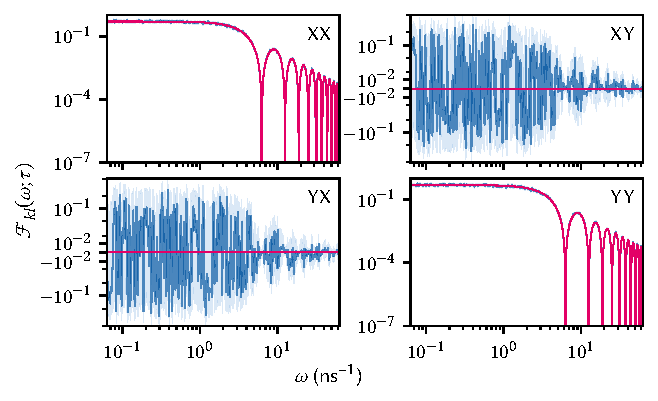
\includegraphics{img/pdf/filter_functions/monte_carlo_FF_Z}
    \caption[\imgsource{img/py/filter_functions/monte_carlo_filter_functions.py}]{
        Non-zero components of the \gls{ff} in the Pauli basis $\mathsf{P}_1$ for the pure dephasing Hamiltonian in \cref{eq:ff:validation:examples:z}.
        Magenta lines are from the cumulant expansion, \cref{eq:ff:filter_function:cumulant:total}, blue lines the mean of the \gls{mc} simulation, \cref{eq:ff:filter_function:monte_carlo}, and light blue shaded areas the \qty{95}{\percent} confidence interval.
        The diagonal elements (XX and YY) agree within the \gls{mc} confidence intervals, with the zeros at $2\pi n/\tau, n\in\{1,2,\dotsc\}$ agreeing down to \num{1e-15} where we can expect numerical errors to be limiting.
        The off-diagonal elements are quite noisy in the \gls{mc} simulation, but fluctuate about the expected value of zero.
    }
    \label{fig:ff:monte_carlo:Z}
\end{figure}

Let us now turn to applying the method to a few select case studies.
First, we consider a pure-dephasing Hamiltonian with
\begin{equation}\label{eq:ff:validation:examples:z}
    \begin{split}
        \Hc(t) &= \Omega\frac{\sz}{2}, \\
        \Hn(t) &= b(t)\frac{\sz}{2}.
    \end{split}
\end{equation}
Specifically, we let the system evolve under the Hamiltonian in \cref{eq:ff:validation:examples:z} for $\tau = \pi/\Omega$ to undergo a $\pi$-rotation around the $z$-axis of the Bloch sphere.
For this model, we expect the cumulant expansion to terminate after the second order because control and noise commute, and hence the interaction-picture noise Hamiltonian, $\Hnt(t)$, always commutes with itself, and therefore the filter-function formalism of \cref{ch:ff:theory} should give the exact result.
\Cref{eq:ff:validation:examples:z} can be solved analytically, and gives rise to an ideal dephasing channel whose \gls{ptm} representation is diagonal, $\liouvUetavg = \diag(1, 1-p, 1-p, 1)$ with $p$ the dephasing probability whose precise value depends on the form of the \gls{psd} $S(\omega)$.
Accordingly, the \gls{ff} $\FF_{kl}(\omega;\tau)$ should be zero everywhere but at $k=l\in\{1, 2\}\equiv\{x, y\}$ for the Pauli basis $\mathsf{P}_1$.
\Cref{fig:ff:monte_carlo:Z} shows the total \enquote{error transfer matrix filter functions} (\cref{eq:ff:filter_function:cumulant:total,eq:ff:filter_function:monte_carlo}) computed with both methods; magenta for the cumulant expansion and blue for the exact \gls{mc} method.
The diagonals agree perfectly within the confidence intervals, while the off-diagonals are dominated by numerical noise in the \gls{mc} approach.
Since the off-diagonals are zero, only the first-order Magnus terms contribute.\sidenote{
    Recall that $\FF\gth{\Delta}(\omega;\tau)$ is anti-symmetric.
}

\begin{figure*}
    \centering
    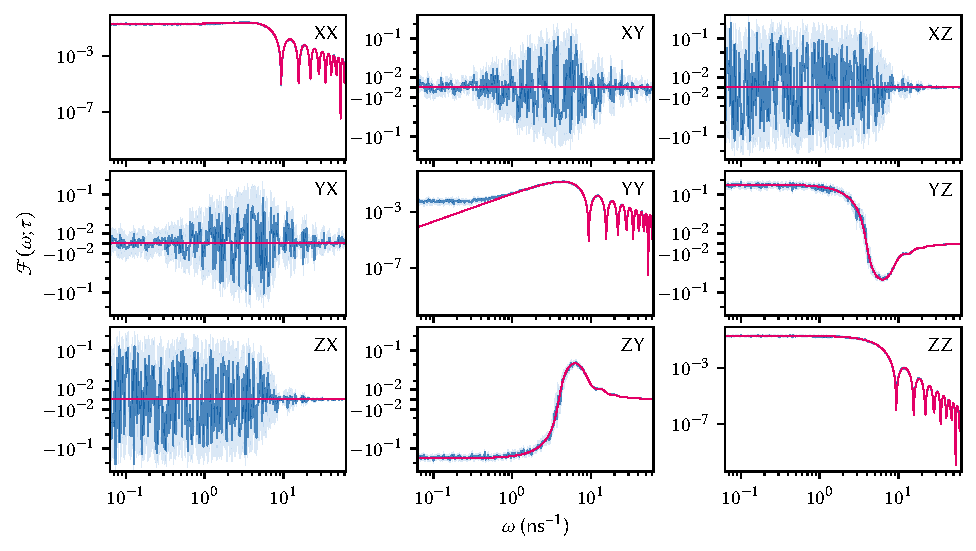
\includegraphics{img/pdf/filter_functions/monte_carlo_FF_X}
    \caption[\imgsource{img/py/filter_functions/monte_carlo_filter_functions.py}]{
        \Glspl{ff} for the non-commuting Hamiltonian in \cref{eq:ff:validation:examples:x}.
        Cumulant expansion calculation is shown in magenta, \gls{mc} in blue with light blue shaded areas the confidence intervals.
        Again, the nominally-zero off-diagonals are susceptible to numerical noise in the \gls{mc} method.
        The YY- and ZZ-terms show a deviation of the cumulant expansion calculation, while all others, including the coherent YZ- and ZY-terms appear to be exact up to the numerical uncertainty.
    }
    \label{fig:ff:monte_carlo:X}
\end{figure*}

The opposite extreme to the pure-dephasing Hamiltonian is obtained when changing the control to be transverse to the noise,
\begin{equation}\label{eq:ff:validation:examples:x}
    \begin{split}
        \Hc(t) &= \Omega\frac{\sx}{2}, \\
        \Hn(t) &= b(t)\frac{\sz}{2}.
    \end{split}
\end{equation}
In this case, control and noise Hamiltonian maximally do not commute at any time ($\Hnt(t)=\sz\cos\Omega t +\i\sy\sin\Omega t$) and we should expect the largest deviations from the exact filter functions in the approximation by truncating the cumulant function after the second order.
\Cref{fig:ff:monte_carlo:X} shows the \gls{ff} for a $\pi$-rotation around the $x$-axis of the Bloch sphere (\ie, $\tau = \pi/\Omega$ once again).
This time, all diagonal elements are nonzero, and the YY-term ($\FF_{22}(\omega;\tau)$ with $\sigma_2\equiv\sy$) displays a deviation between cumulant expansion and \gls{mc} simulation towards low frequencies!
This is exactly what we would expect according to \citet{Fox1976}, namely that the more correlated the noise is, the larger contributions from higher orders will be.\sidenote{
    Quasistatic noise is perfectly correlated---it assumes a single value for all times.
}
Also deviating is the ZZ-term, although not towards DC but where the filter function computed from the approximated cumulant function drops to zero.
By contrast, the XX-term shows good agreement between both methods.
Finally, two non-diagonal elements are nonzero, YZ and ZY, anti-symmetric terms which arise from the second-order Magnus and incur coherent errors.
For these, the cumulant approximation is excellent, showing no deviation within the confidence intervals.

\begin{figure*}
    \centering
    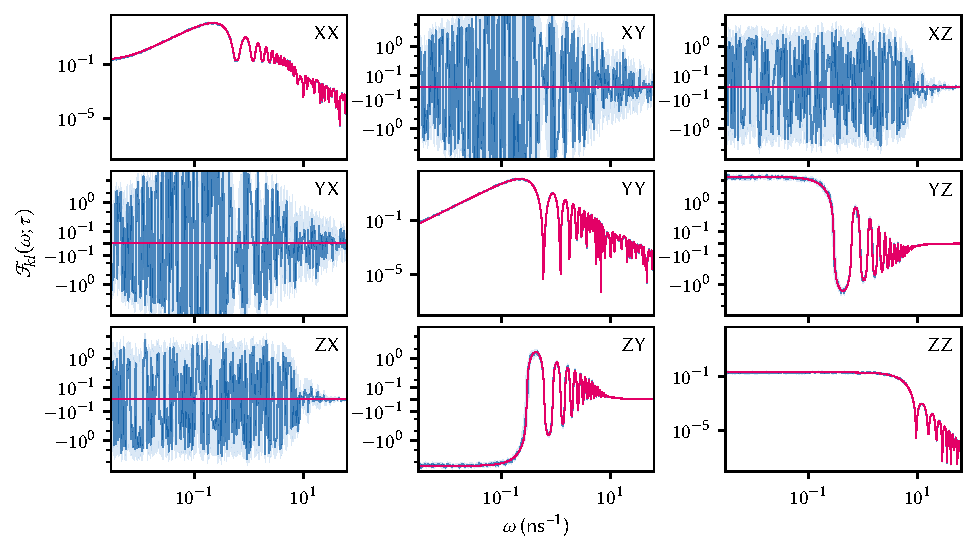
\includegraphics{img/pdf/filter_functions/monte_carlo_FF_spin_echo}
    \caption[\imgsource{img/py/filter_functions/monte_carlo_filter_functions.py}]{
        \Glspl{ff} for the \gls{se} Hamiltonian in \cref{eq:ff:validation:examples:se}.
        Cumulant expansion calculation is shown in magenta, \gls{mc} in blue with light blue shaded areas the confidence intervals.
        Both coherent and incoherent terms show excellent agreement between both methods.
    }
    \label{fig:ff:monte_carlo:se}
\end{figure*}

Finally, as a last example we consider the prototypical filter-function use case: the \acrfull{se}.
Here, the qubit idles for a time $\tau_{0}$ both before and after a $\pi$ rotation around the $x$-axis of the Bloch sphere, so that the Hamiltonian is given by
\begin{equation}\label{eq:ff:validation:examples:se}
    \begin{split}
        \Hc(t) &= \Omega(t)\frac{\sx}{2}, \\
        \Hn(t) &= b(t)\frac{\sz}{2},
    \end{split}
\end{equation}
with $\Omega(t) = \pi/\tau_\pi$ if $t\in[\tau_0, \tau_0+\tau_\pi]$ and zero else.
This pulse sequence is known to cancel quasistatic dephasing noise as the phase picked up on the equator of the Bloch sphere during the first period of free evolution is exactly cancelled by the phase picked up during the second period after the $\pi$-pulse.
Since the previous example demonstrated that the filter-function formalism based on the second-order cumulant expansion neglects contributions from higher orders in the case of transverse noise, we might expect the \gls{se} sequence to show similar behavior.
\Cref{fig:ff:monte_carlo:se} shows the results of the simulation.
The picture is similar -- albeit more complex -- to before, with nominally-zero terms suffering from numerical noise.
However, in contrast to the simple $\pi$-pulse Hamiltonian in \cref{eq:ff:validation:examples:x,fig:ff:monte_carlo:X}, the YY and ZZ terms show excellent agreement between the exact \gls{mc} method and the cumulant expansion.
We may speculate that the higher-order contributions not captured by the cumulant method in the previous case drop out due to the symmetry of the Hamiltonian.

In conclusion, we have developed a method to numerically compute the exact filter functions of the quantum process description of arbitrary Gaussian noise, and compared the thus obtained filter functions with those from the second-order truncation of the \gls{me} and cumulant expansions given in \cref{ch:ff:theory}.
The approach samples the Liouville-space filter function at discrete frequencies $\omega_i$ by simulating the unitary dynamics under monochromatic noise at that frequencies and averaging over the outcomes.
We found excellent agreement between the nominally exact and approximate methods in the case of commuting noise as well as the \gls{se} \gls{dd} sequence.
For non-commuting noise, we observed the expected deviation at very low frequencies that arises from non-vanishing higher order cumulants.

Rather than random sampling using \gls{mc}, this average could also be performed deterministically as the expectation value over the probability distributions governing $A_i$ and $\phi$,
\begin{equation}
    \mathbb{E}_{A_i,\phi}[\liouvU] = \int\dd{x}\rho_{A_i}(x)\int\dd{y}\rho_{\phi}(y)\liouvU[x, y],
\end{equation}
where we wrote $\liouvU[x, y]$ for the Liouville representation of the propagator for single $x$ and $y$ drawn from their respective distributions, and $\mathbb{E}_X[A]$ denotes the expectation value of an observable $A$ with respect to the random variable $X$ with probability density function $\rho_X$.
This technique allows the expectation value $\mathbb{E}[\liouvU]\equiv\ev{\liouvU}$ to be evaluated to arbitrary precision numerically, but is typically less efficient than \gls{mc}.
It would be interesting to see if the numerical noise observed in off-diagonal elements of the filter functions in \cref{fig:ff:monte_carlo:Z,fig:ff:monte_carlo:X,fig:ff:monte_carlo:se} persists with this method.
